\documentclass[12pt]{article}
\usepackage[utf8]{inputenc}
\usepackage[T2A]{fontenc}
\usepackage[russian]{babel}
\usepackage{amsmath}
\usepackage{graphicx}
\usepackage{geometry}

\geometry{a4paper, left=2cm, right=2cm, top=2cm, bottom=2cm}

\title{Краткий отчёт по решению}
\author{Васильев Павел Петрович \\ группа 303 ВМК МГУ}

\begin{document}
	
	\maketitle
	
	\begin{abstract}
	В данном репозитории представлен алгоритм решения системы линейных алгебраических уравнений методом Холецкого на языке программирования C++. Были проведены тесты для $x \in \mathcal{R}^n: \; x \in \mathcal{U}_{[-1, 1]}$, а также использовались вещественные числа разного порядка точности: float16, float32, float64. Для всех тестов были вычислены максимальные и средние нормы невязки, погрешности решений и времени работы. Использована норма $||*||_{\infty}$. В работе были использованы языки C++ для вычислений и Python для анализа результатов.
	
	Ссылка на репозиторий:  https://github.com/GoodDay-lab/cholesky-decomposition
	\end{abstract}
	
	\section{Постановка задачи}
	Перед нами поставлена задача решить следующую систему линейных уравнений:
	
	\begin{align}
	\mathnormal{A} \in \mathcal{R}^{n \times n}: \; A^T = A, \; A > 0; \; b \in \mathcal{R}^n \rightarrow
	Ax = b
	\end{align}
		
	\section{Почему не Гаусс?}
		Одним из первых алгоритмов для решения подобных систем можно назвать алгоритм Гаусса, в сущности, это нахождение LU разложения для матрицы $A$. Данный алгоритм неустойчив при небольшом значении диагонального элемента матрицы (близком к машинному нулю), к примеру:
	\[
	A = 
	\begin{bmatrix}
		10^{-8} & 1 .0 \\
		1.0 & 1.0 \\
	\end{bmatrix}
	\] 
	\[
	\tilde{L} =
	\begin{bmatrix}
		1.0 & 0 \\
		10^{-8} & 1.0 \\
	\end{bmatrix}
	\;\;\;\;
	\tilde{U} =
	\begin{bmatrix}
		10^{-8} & 1.0 \\
		0 & -10^{-8} \\
	\end{bmatrix}
	\]
	Тогда 
	\[
	\tilde{L} \tilde{U} - A =
	\begin{bmatrix}
		0 & 0 \\
		0 & 1 \\
	\end{bmatrix}
	\]
	
	С другой стороны, у нас есть алгоритм Холецкого, который лишён данной проблемы, это объясняется тем, что $c_{kk} = \sqrt{a_{kk} - (\dots)}$, даже если $a_{kk}$ близко к минимально представимому на машине типу float, деление всё равно происходит на его корень, что больше, чем изначальное число. Более подробное обоснование можно прочесть в учебнике E.E.Тыртышникова "Методы Численного Анализа".
	
	\section{Алгоритм Холецкого для решения СЛАУ}
	Вернёмся к изначальным условиям задачи (1).
	
	Рассмотрим следующее уравнение:
	\[
	\begin{bmatrix}
		a_{11} & a_{12} & a_{13} \\
		a_{21} & a_{22} & a_{23} \\
		a_{31} & a_{32} & a_{33} \\
	\end{bmatrix}
	=
	\begin{bmatrix}
		c_{11} & 0 & 0 \\
		c_{21} & c_{22} & 0 \\
		c_{31} & c_{32} & c_{33} \\
	\end{bmatrix}
	\begin{bmatrix}
		c_{11} & c_{21} & c_{31} \\
		0 & c_{22} & c_{32} \\
		0 & 0 & c_{33} \\
	\end{bmatrix}
	\]
	
	Попробуем вычислить коэффиценты:
	\[
		c_{11} = \sqrt{a_{11}}, \;\; c_{21} = \frac{a_{21}}{c_{11}}, \;\; c_{31} = \frac{a_{31}}{c_{11}} 
	\]
	\[
		c_{22} = \sqrt{a_{22} - c_{21}^2}, \;\; c_{32} = \frac{a_{32} - c_{31} c_{21}}{c_{22}}
	\]
	\[
		c_{33} = \sqrt{a_{33} - c_{31}^2 - c_{32}^2}
	\]
	
	Обобщая для любого $n$, получим:
	
	\begin{align}
		c_{kk} = \left( a_{kk} - \sum_{j=1}^{k-1} c_{kj}^2)^{\frac{1}{2}} \right) \\
		c_{ik} = \frac{\left( a_{ik} - \sum_{j=1}^{k-1} c_{ij} c_{kj} \right)}{c_{kk}}, \; \forall  1 \le i < k
	\end{align}
	
	Хорошо, мы получили удобное представление $A = L L^T$ из треугольных матриц $L$, а для них мы можем легко решить систему уравнений строчка за строчкой со сложность $O(n^2)$.  Что ж тогда давайте пользоваться принципом разделяй-и-властвуй и решим две более простые системы линейных уравнений
	
	\begin{align}
	A x = b \Longrightarrow L L^T x = b \Longrightarrow  
	\begin{cases}
		L y = b \\
		L^T x = y \\
	\end{cases}
	\end{align}
	
	Что ж, отлично! Решение этих двух систем в разы проще, поскольку для каждого нового $y_i$ мы можем пользоваться ранее подсчитанными $y_1,\, \cdots,\, y_{i-1}$. Теперь мы сможем легко решить данную систему, время писать код.
	
	
	\section{Результаты}
	Полученные значения времени работы и погрешности измерений представлены на графиках ниже. К примеру, один и тот же алгоритм работает по-разному для разных типов данных, наименьшая величина достигается на f32 (\ref{fig:t-t3-f32}), а наибольшая, как ни странно, на f16 (\ref{fig:t-t3-f16}).
	
	Так же, при увеличении типа float увеличивается и качество работы алгоритма, достаточно сравнить норму невязки на f16 (\ref{fig:t-t1-f16}) и f64 (\ref{fig:t-t1-f64}).
	
	\section{Выводы}
	У нас получилось реализовать устойчивый алгоритм для решения системы СЛАУ методом Холецкого на языке программирования С++. Средняя скорость алгоритма составляет 12 мс для матрицы $100 \times 100$, в зависимости от типа вещественного числа. Код доступен по ссылке в аннотации.
	
	\section{Графики}
	
	\begin{figure}[h]
		\centering
		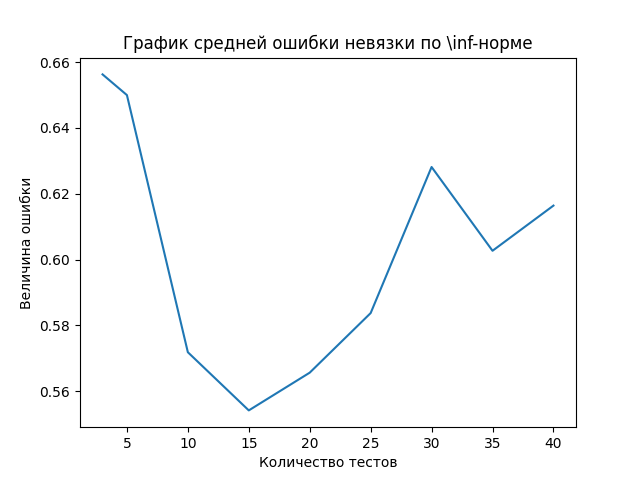
\includegraphics[width=16cm]{"../plots/plot-total-t1-f16.png"}
		\caption{f16}
		\label{fig:t-t1-f16}
	\end{figure}

	\begin{figure}[h]
		\centering
		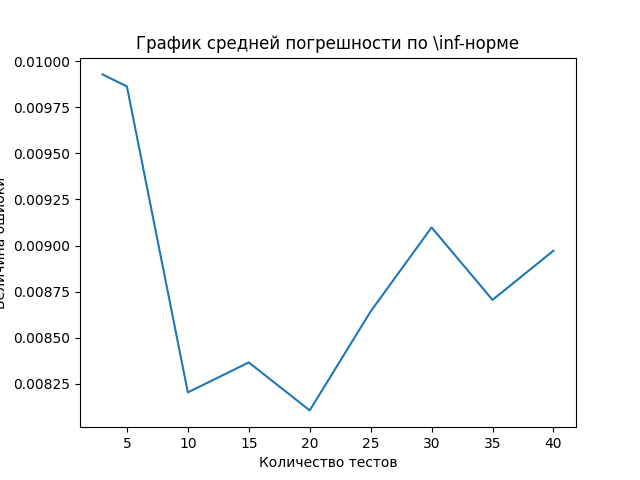
\includegraphics[width=16cm]{"../plots/plot-total-t2-f16.png"}
		\caption{f16}
		\label{fig:t-t2-f16}
	\end{figure}
	
	\begin{figure}[h]
		\centering
		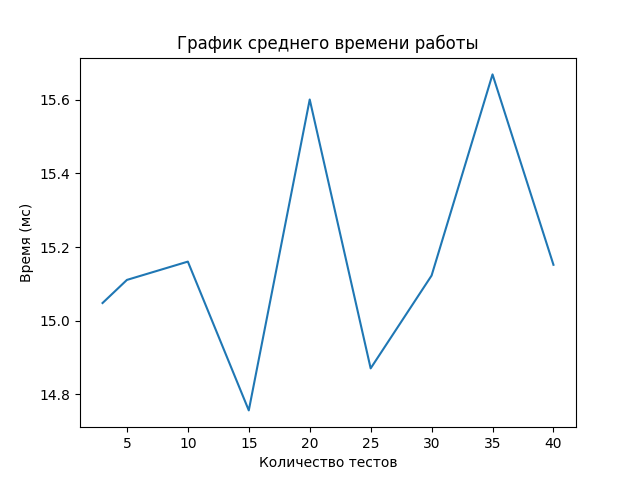
\includegraphics[width=16cm]{"../plots/plot-total-t3-f16.png"}
		\caption{f16}
		\label{fig:t-t3-f16}
	\end{figure}
	
	\begin{figure}[h]
		\centering
		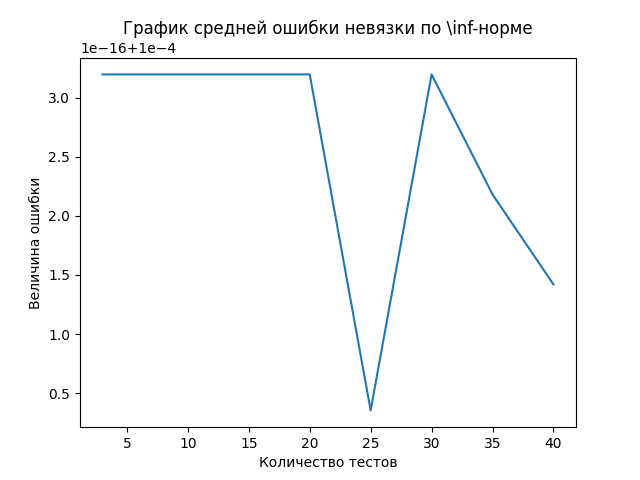
\includegraphics[width=16cm]{"../plots/plot-total-t1-f32.png"}
		\caption{f32}
		\label{fig:t-t1-f32}
	\end{figure}
	
	\begin{figure}[h]
		\centering
		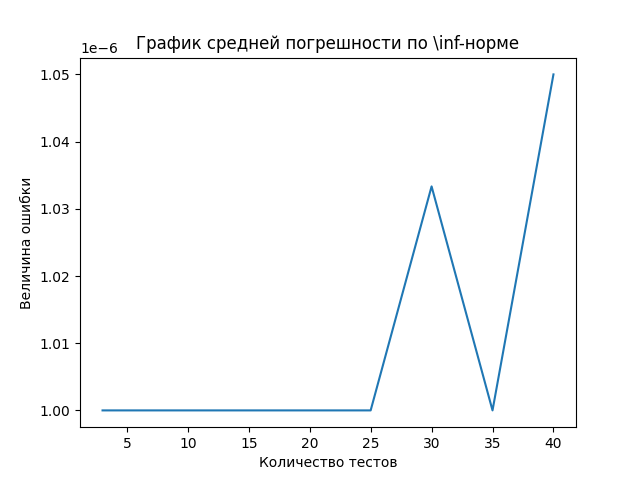
\includegraphics[width=16cm]{"../plots/plot-total-t2-f32.png"}
		\caption{f32}
		\label{fig:t-t2-f32}
	\end{figure}
	
	\begin{figure}[h]
		\centering
		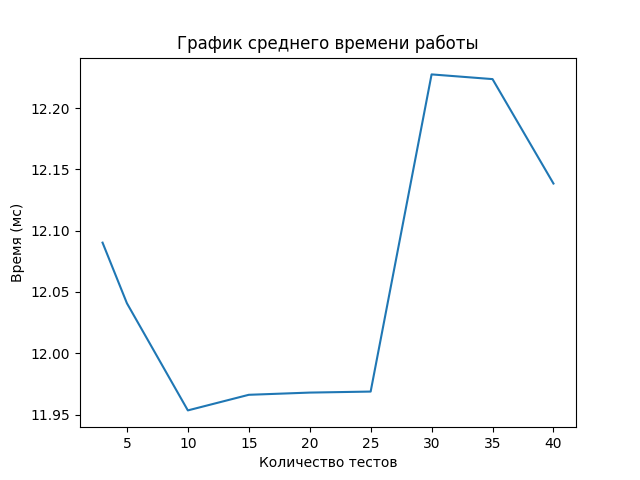
\includegraphics[width=16cm]{"../plots/plot-total-t3-f32.png"}
		\caption{f32}
		\label{fig:t-t3-f32}
	\end{figure}
	
	\begin{figure}[h]
		\centering
		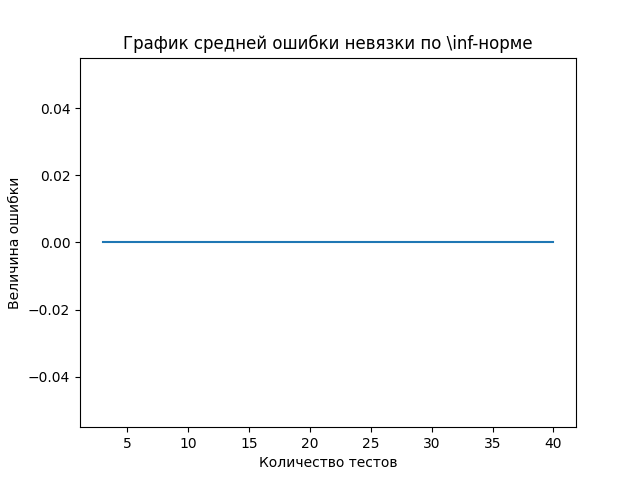
\includegraphics[width=16cm]{"../plots/plot-total-t1-f64.png"}
		\caption{f64}
		\label{fig:t-t1-f64}
	\end{figure}
	
	\begin{figure}[h]
		\centering
		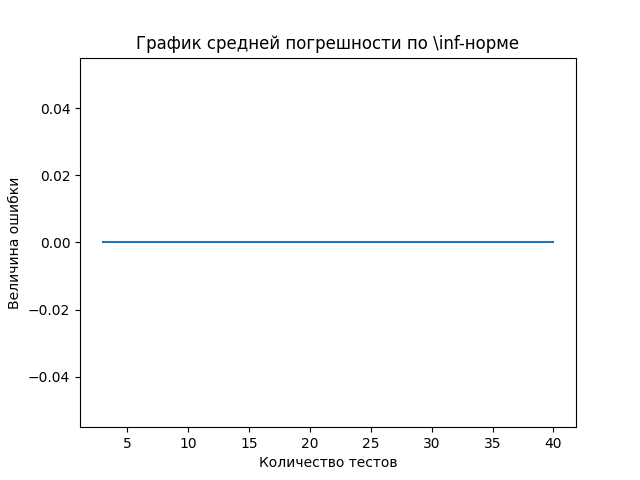
\includegraphics[width=16cm]{"../plots/plot-total-t2-f64.png"}
		\caption{f64}
		\label{fig:t-t2-f64}
	\end{figure}
	
	\begin{figure}[h]
		\centering
		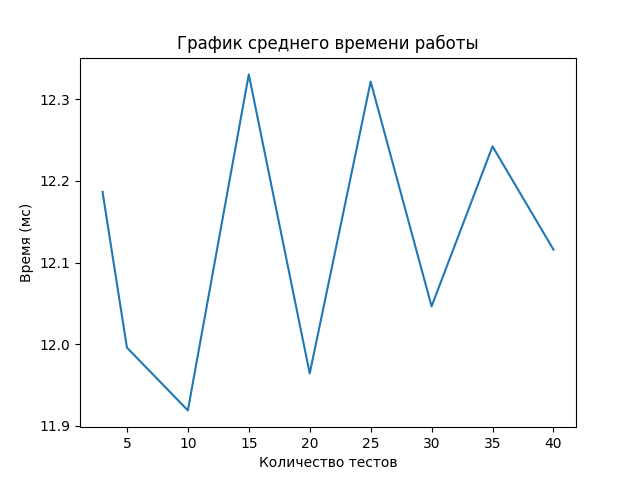
\includegraphics[width=16cm]{"../plots/plot-total-t3-f64.png"}
		\caption{f64}
		\label{fig:t-t3-f64}
	\end{figure}
	
\end{document}